\documentclass[a4paper,11pt]{article}

% Packages
\usepackage{listings}
\lstset{
    breaklines=true, % Break long lines
    language=SQL, % Set language for syntax highlighting
    basicstyle=\small, % Set the font size
    numbers=none, % No line numbers
    frame=single % Add a frame around the code
}
\usepackage{placeins}
\usepackage{float}
\usepackage{caption}
\usepackage[utf8]{inputenc}
\usepackage{amsmath}
\usepackage{graphicx}
\usepackage{geometry}
\usepackage{enumitem}
\geometry{a4paper, margin=1in}

% Title and Author
\title{Project 2}
\author{Ahmed Tlili, Leon Petrinos, Mathilde Peruzzo}
\date{\today}

\begin{document}

\maketitle

\section{ER Diagram}
\begin{figure}[h]
    \centering
    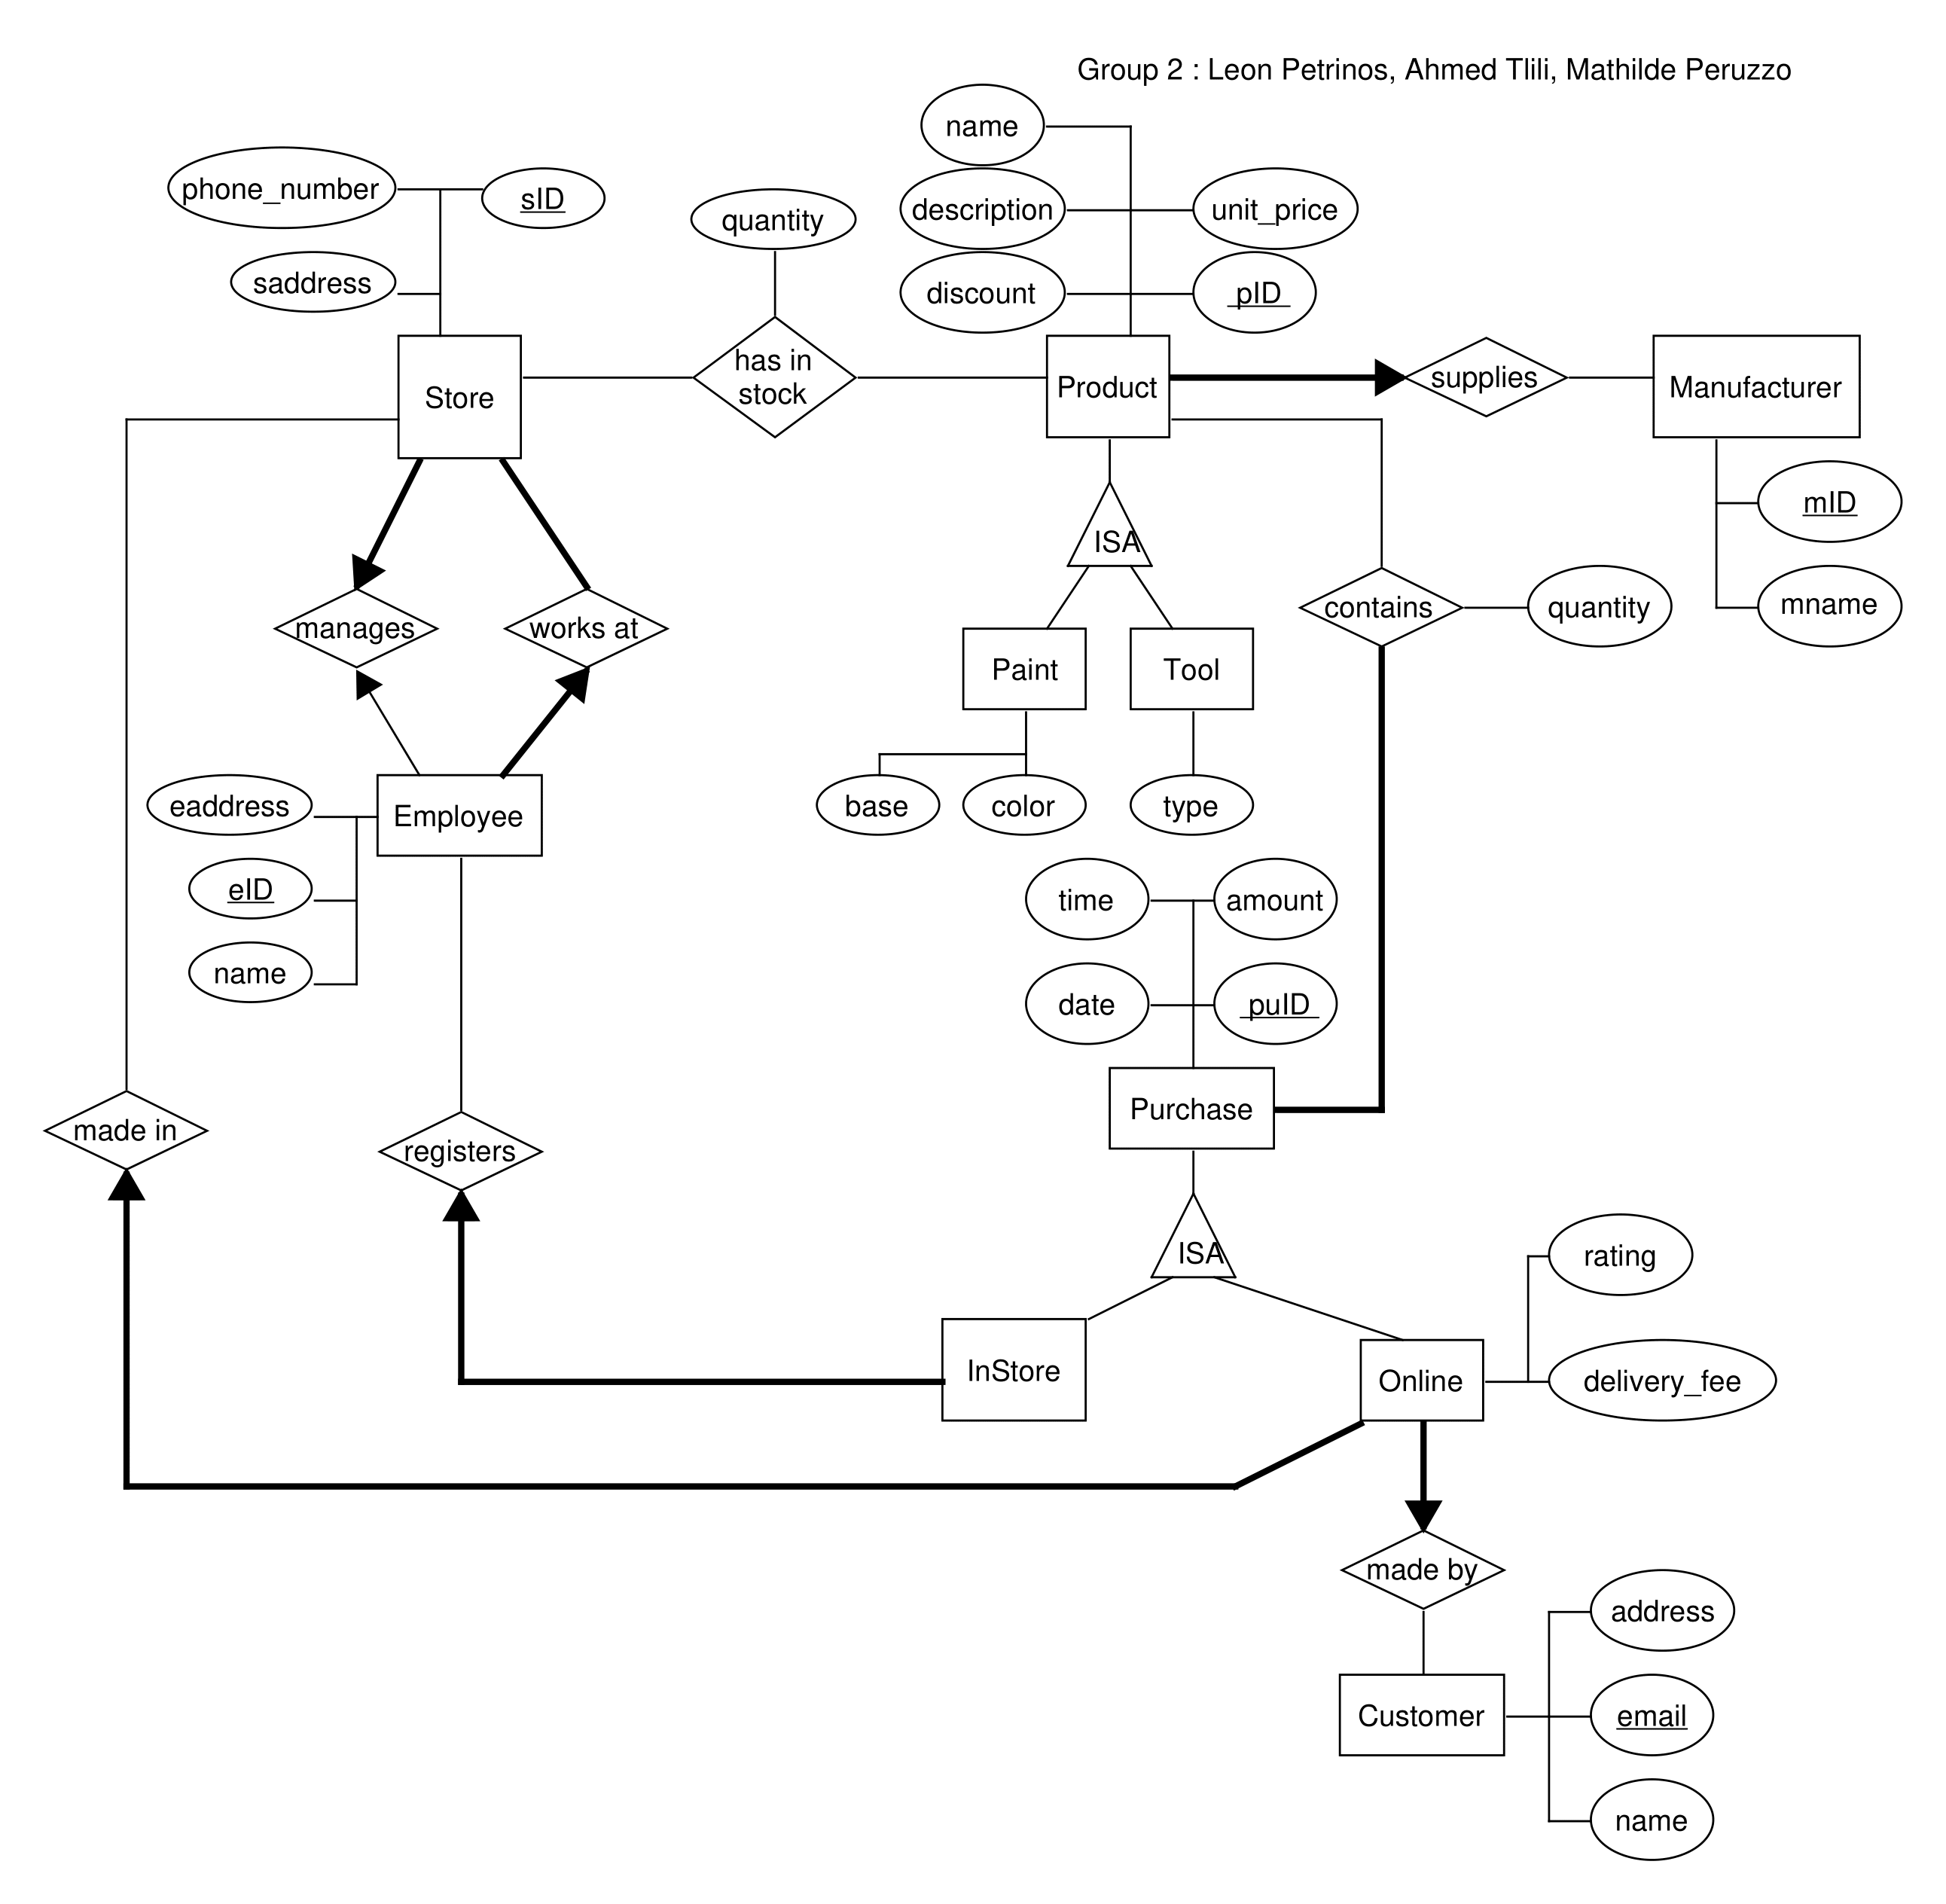
\includegraphics[width=0.8\textwidth]{ER.png}
    \caption{ER Diagram}
\end{figure}

\section{Relational Schema}
\begin{itemize}
    \item \textbf{Store}(\underline{s\_id}, s\_address, phone\_number, manager\_id UNIQUE NOT NULL)\\
        FOREIGN KEY(manager\_id) REFERENCES Employee(employee\_id)
    \item \textbf{Employee}(\underline{e\_id}, e\_name, s\_id)\\
        FOREIGN KEY(s\_id) REFERENCES Store(s\_id)
    \item \textbf{Manufacturer}(\underline{m\_id}, m\_name)
    \item \textbf{Product}(\underline{p\_id}, p\_name NOT NULL, unit\_price NOT NULL, description,\\ discount\_percentage, m\_id NOT NULL)\\
        FOREIGN KEY(m\_id) REFERENCES Manufacturer(m\_id)
    \item \textbf{Paint}(\underline{p\_id}, base, color)\\
        FOREIGN KEY(p\_id) REFERENCES Product(p\_id)
    \item \textbf{Tool}(\underline{p\_id}, type)
    \item \textbf{Has\_in\_stock}(\underline{p\_id}, \underline{s\_id}, quantity NOT NULL )\\
        FOREIGN KEY(p\_id) REFERENCES Product(p\_id)\\
        FOREIGN KEY(s\_id) REFERENCES Store(s\_id)
    \item \textbf{Customer}(\underline{email}, c\_name, c\_address NOT NULL)\\
        PRIMARY KEY(email)
    \item \textbf{Purchase}(\underline{p\_id}, amount NOT NULL, p\_date NOT NULL, p\_time NOT NULL)
    \item \textbf{Contains\_purchase}(\underline{p\_id}, \underline{product\_id}, quantity NOT NULL)\\
        FOREIGN KEY(p\_id) REFERENCES Purchase(p\_id)\\
        FOREIGN KEY(product\_id) REFERENCES Product(p\_id)
    \item \textbf{Instore}(\underline{p\_id}, \underline{e\_id})\\
        FOREIGN KEY(p\_id) REFERENCES Purchase(p\_id)\\
        FOREIGN KEY(e\_id) REFERENCES Employee(e\_id)
    \item \textbf{Online}(\underline{p\_id}, rating, delivery\_fee NOT NULL, email NOT NULL)\\
        FOREIGN KEY(p\_id) REFERENCES Purchase(p\_id)\\
        FOREIGN KEY(email) REFERENCES Customer(email)


\end{itemize}

\section{Pending Constraints}
\begin{itemize}
    \item A store should have at least one employee.
    \item A purchase should have at least one product.
    \item Cannot have store manager\_id referencing a row in the Employee table.\\
        As here we have two tables referencing each other (STORE, EMPLOYEE).\\
        One of them has to drop the foreign key constraint.

\end{itemize}

\section{SQL Queries}
\subsection*{Query 1}
\begin{enumerate}[label=(\alph*)]
    \item List the id and address of every store with the respective quantities of the products (with p\_id = 3) they have in stock.
    \item
        \begin{lstlisting}
        SELECT STORE.s_id, s_address, COALESCE(quantity, 0) AS quantity
        FROM STORE
        LEFT JOIN HAS_IN_STOCK
        ON STORE.s_id = HAS_IN_STOCK.s_id AND HAS_IN_STOCK.p_id = 3
        ORDER BY STORE.s_id ASC;
        \end{lstlisting}
    \item
\end{enumerate}
\begin{figure}[H]
    \centering
    \includegraphics[width=0.8\textwidth]{query1.png}
    \caption{Query 1 result}
\end{figure}

\subsection*{Query 2}
\begin{enumerate}[label=(\alph*)]
    \item List the total amount of money spent by each customer in the store with id = 1.\\
        Output should include the customer's email and the total amount of money spent.
    \item
        \begin{lstlisting}
        SELECT CUSTOMER.email, COALESCE(SUM(amount), 0) AS total_amount
        FROM CUSTOMER
        LEFT JOIN ONLINE ON CUSTOMER.email = ONLINE.email
        LEFT JOIN PURCHASE ON ONLINE.p_id = PURCHASE.p_id
        LEFT JOIN STORE ON ONLINE.s_id = STORE.s_id
        GROUP BY CUSTOMER.email
        ORDER BY email ASC;
        \end{lstlisting}
    \item
\end{enumerate}
\begin{figure}[H]
    \centering
    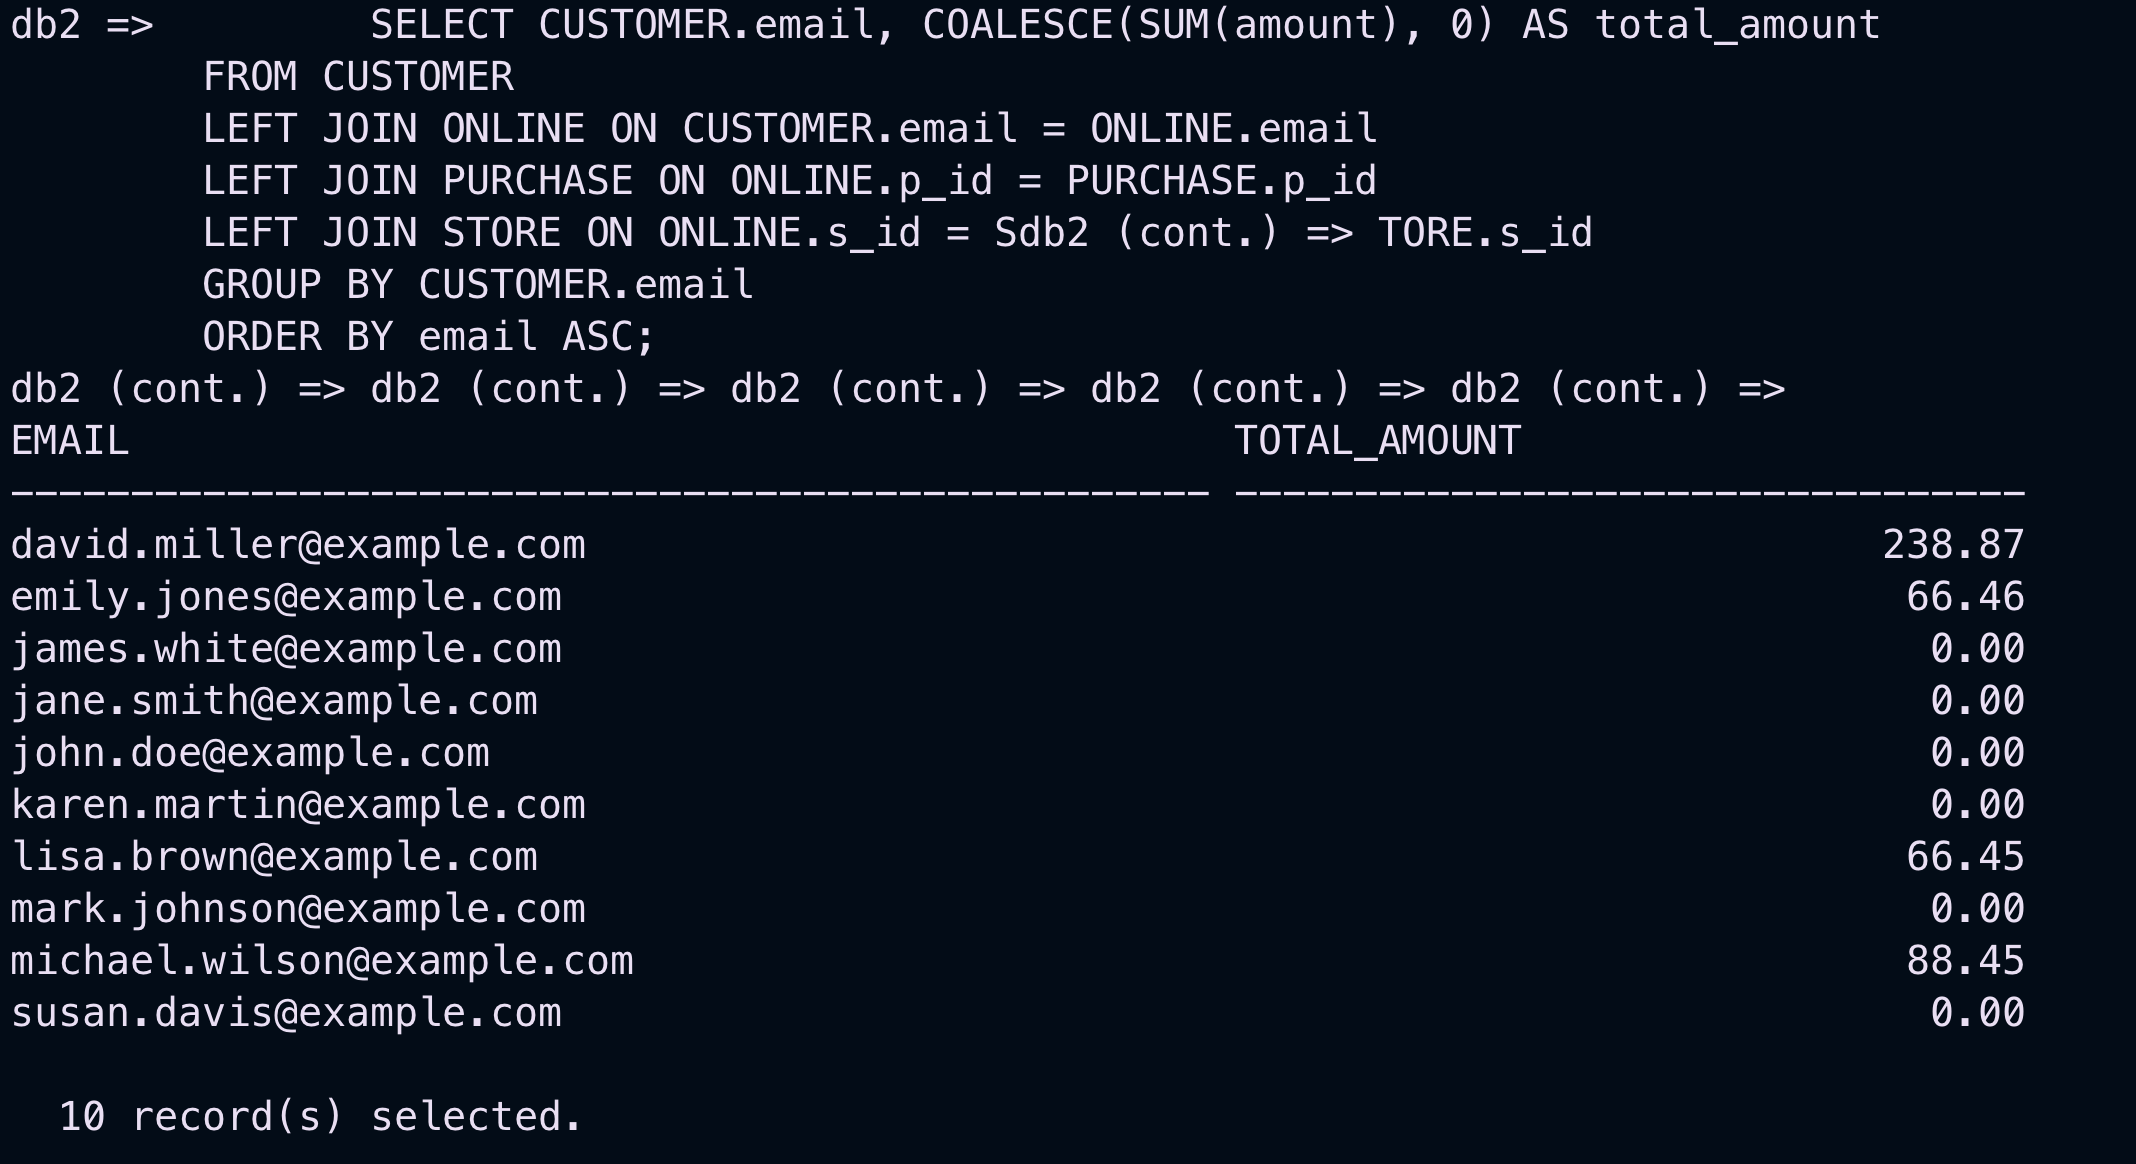
\includegraphics[width=0.8\textwidth]{Query2.png}
    \caption{Query 2 result}
\end{figure}

\subsection*{Query 3}
\begin{enumerate}[label=(\alph*)]
    \item List the id of the biggest in-store purchase made by each store.\\
        Output should include the store id, address and the purchase amount.
    \item
        \begin{lstlisting}
        SELECT STORE.s_id, s_address, COALESCE(MAX(amount), 0) AS max_purchase_amount
        FROM STORE
        LEFT JOIN EMPLOYEE ON STORE.s_id = EMPLOYEE.s_id
        LEFT JOIN INSTORE ON EMPLOYEE.e_id = INSTORE.e_id
        LEFT JOIN PURCHASE ON INSTORE.p_id = PURCHASE.p_id
        GROUP BY STORE.s_id, s_address
        ORDER BY STORE.s_id ASC;
        \end{lstlisting}
    \item
\end{enumerate}
\begin{figure}[H]
    \centering
    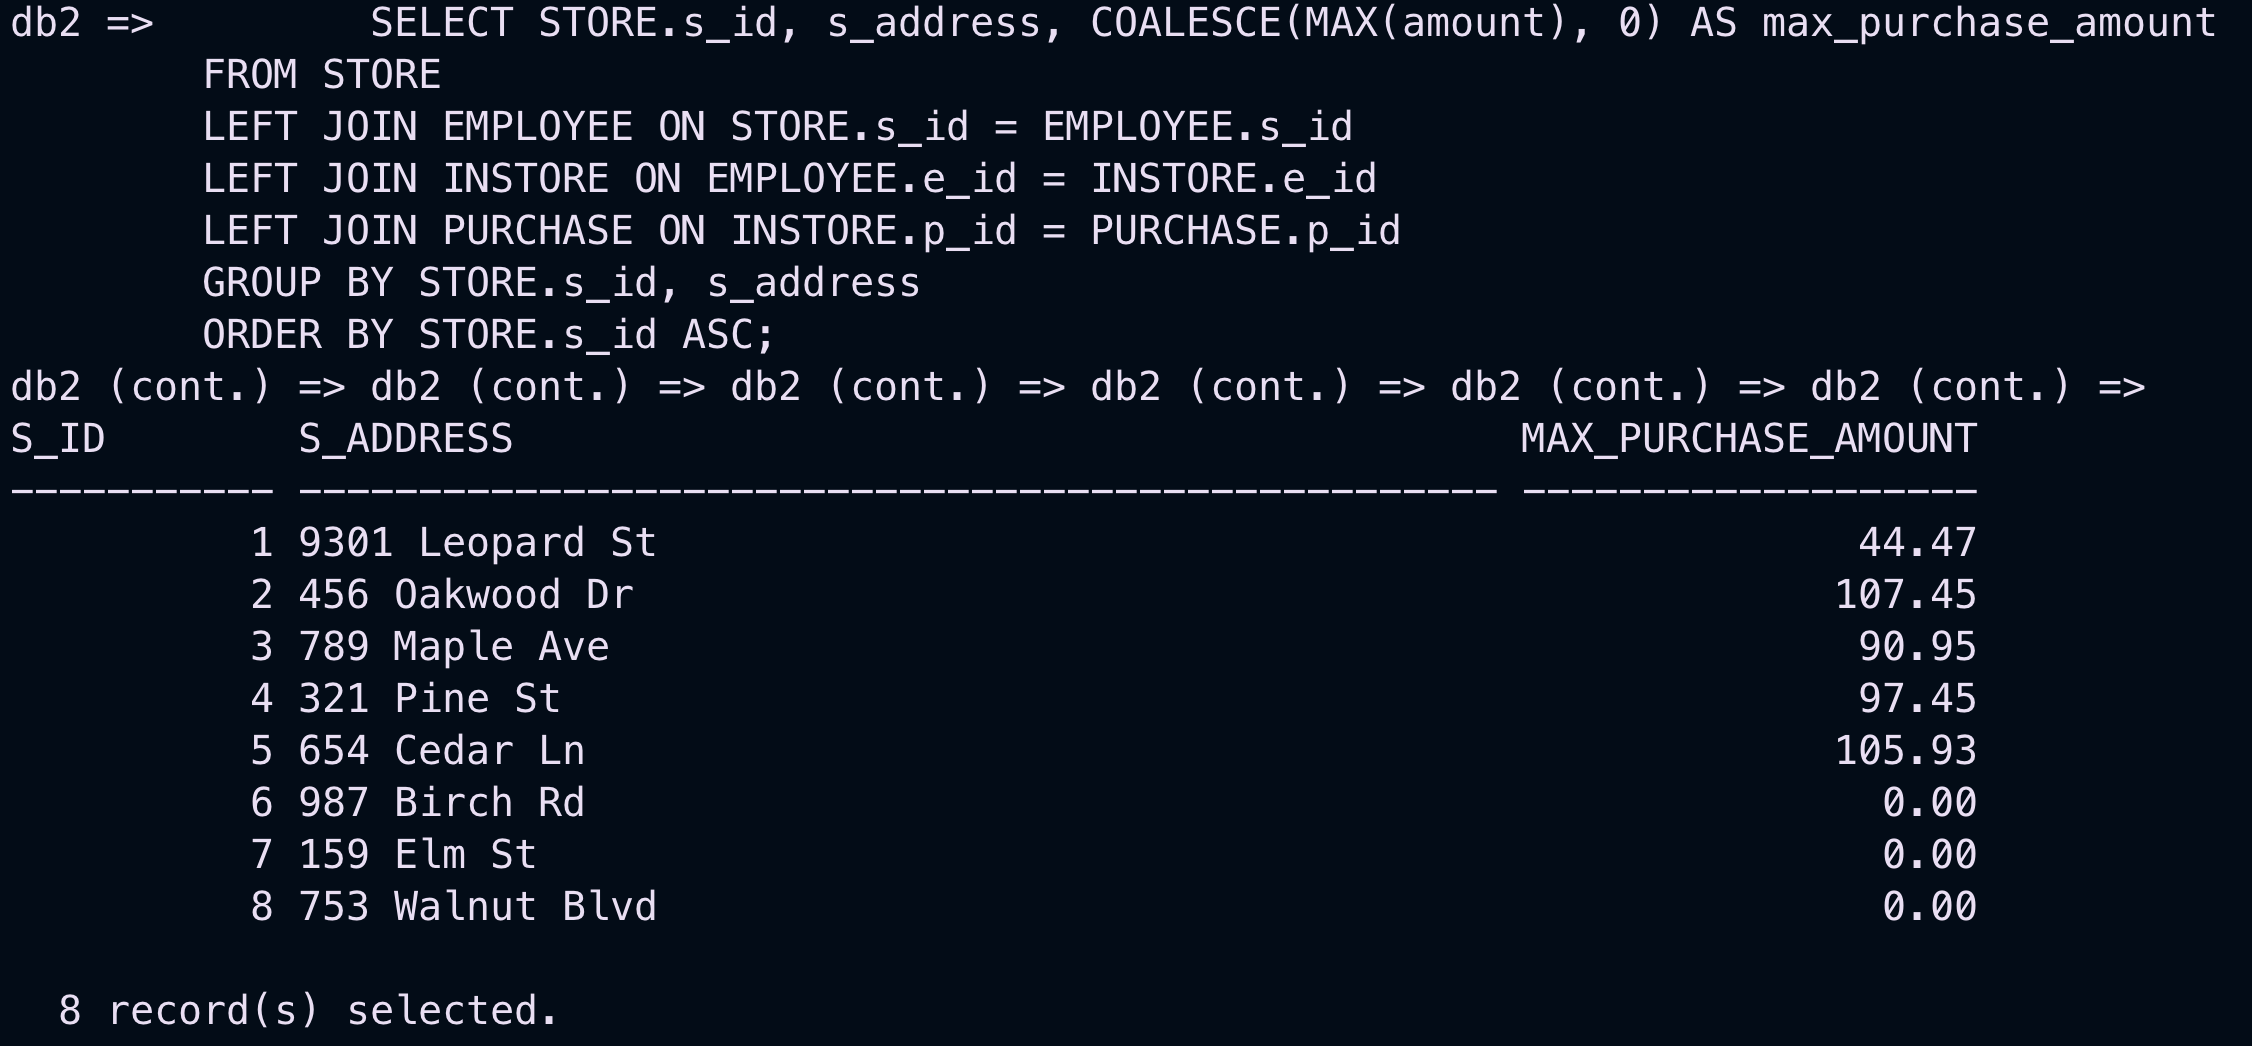
\includegraphics[width=0.8\textwidth]{Query3.png}
    \caption{Query 3 result}
\end{figure}

\subsection*{Query 4}
\begin{enumerate}[label=(\alph*)]
    \item List the id and address of every store and the corresponding money ever spent at that store.
    \item
        \begin{lstlisting}
        WITH TEMP_INSTORE AS (
        SELECT STORE.s_id, s_address, COALESCE(SUM(amount), 0) AS total_amount
            FROM STORE
            LEFT JOIN EMPLOYEE ON STORE.s_id = EMPLOYEE.s_id
            LEFT JOIN INSTORE ON EMPLOYEE.e_id = INSTORE.e_id
            LEFT JOIN PURCHASE ON INSTORE.p_id = PURCHASE.p_id
            GROUP BY STORE.s_id, s_address
        ),
        TEMP\_ONLINE AS (
            SELECT STORE.s_id, s_address, COALESCE(SUM(amount), 0) AS total_amount
            FROM STORE
            LEFT JOIN ONLINE ON STORE.s_id = ONLINE.s_id
            LEFT JOIN PURCHASE ON ONLINE.p_id = PURCHASE.p_id
            GROUP BY STORE.s_id, s_address
        )
        SELECT TEMP_INSTORE.s_id, TEMP_INSTORE.s_address,
        TEMP_INSTORE.total_amount + TEMP_ONLINE.total_amount AS total_amount
        FROM TEMP_INSTORE
        LEFT JOIN TEMP_ONLINE ON TEMP_INSTORE.s_id = TEMP_ONLINE.s_id
        ORDER BY TEMP_INSTORE.s_id ASC;
        \end{lstlisting}

    \item
\end{enumerate}
\begin{figure}[H]
    \centering
    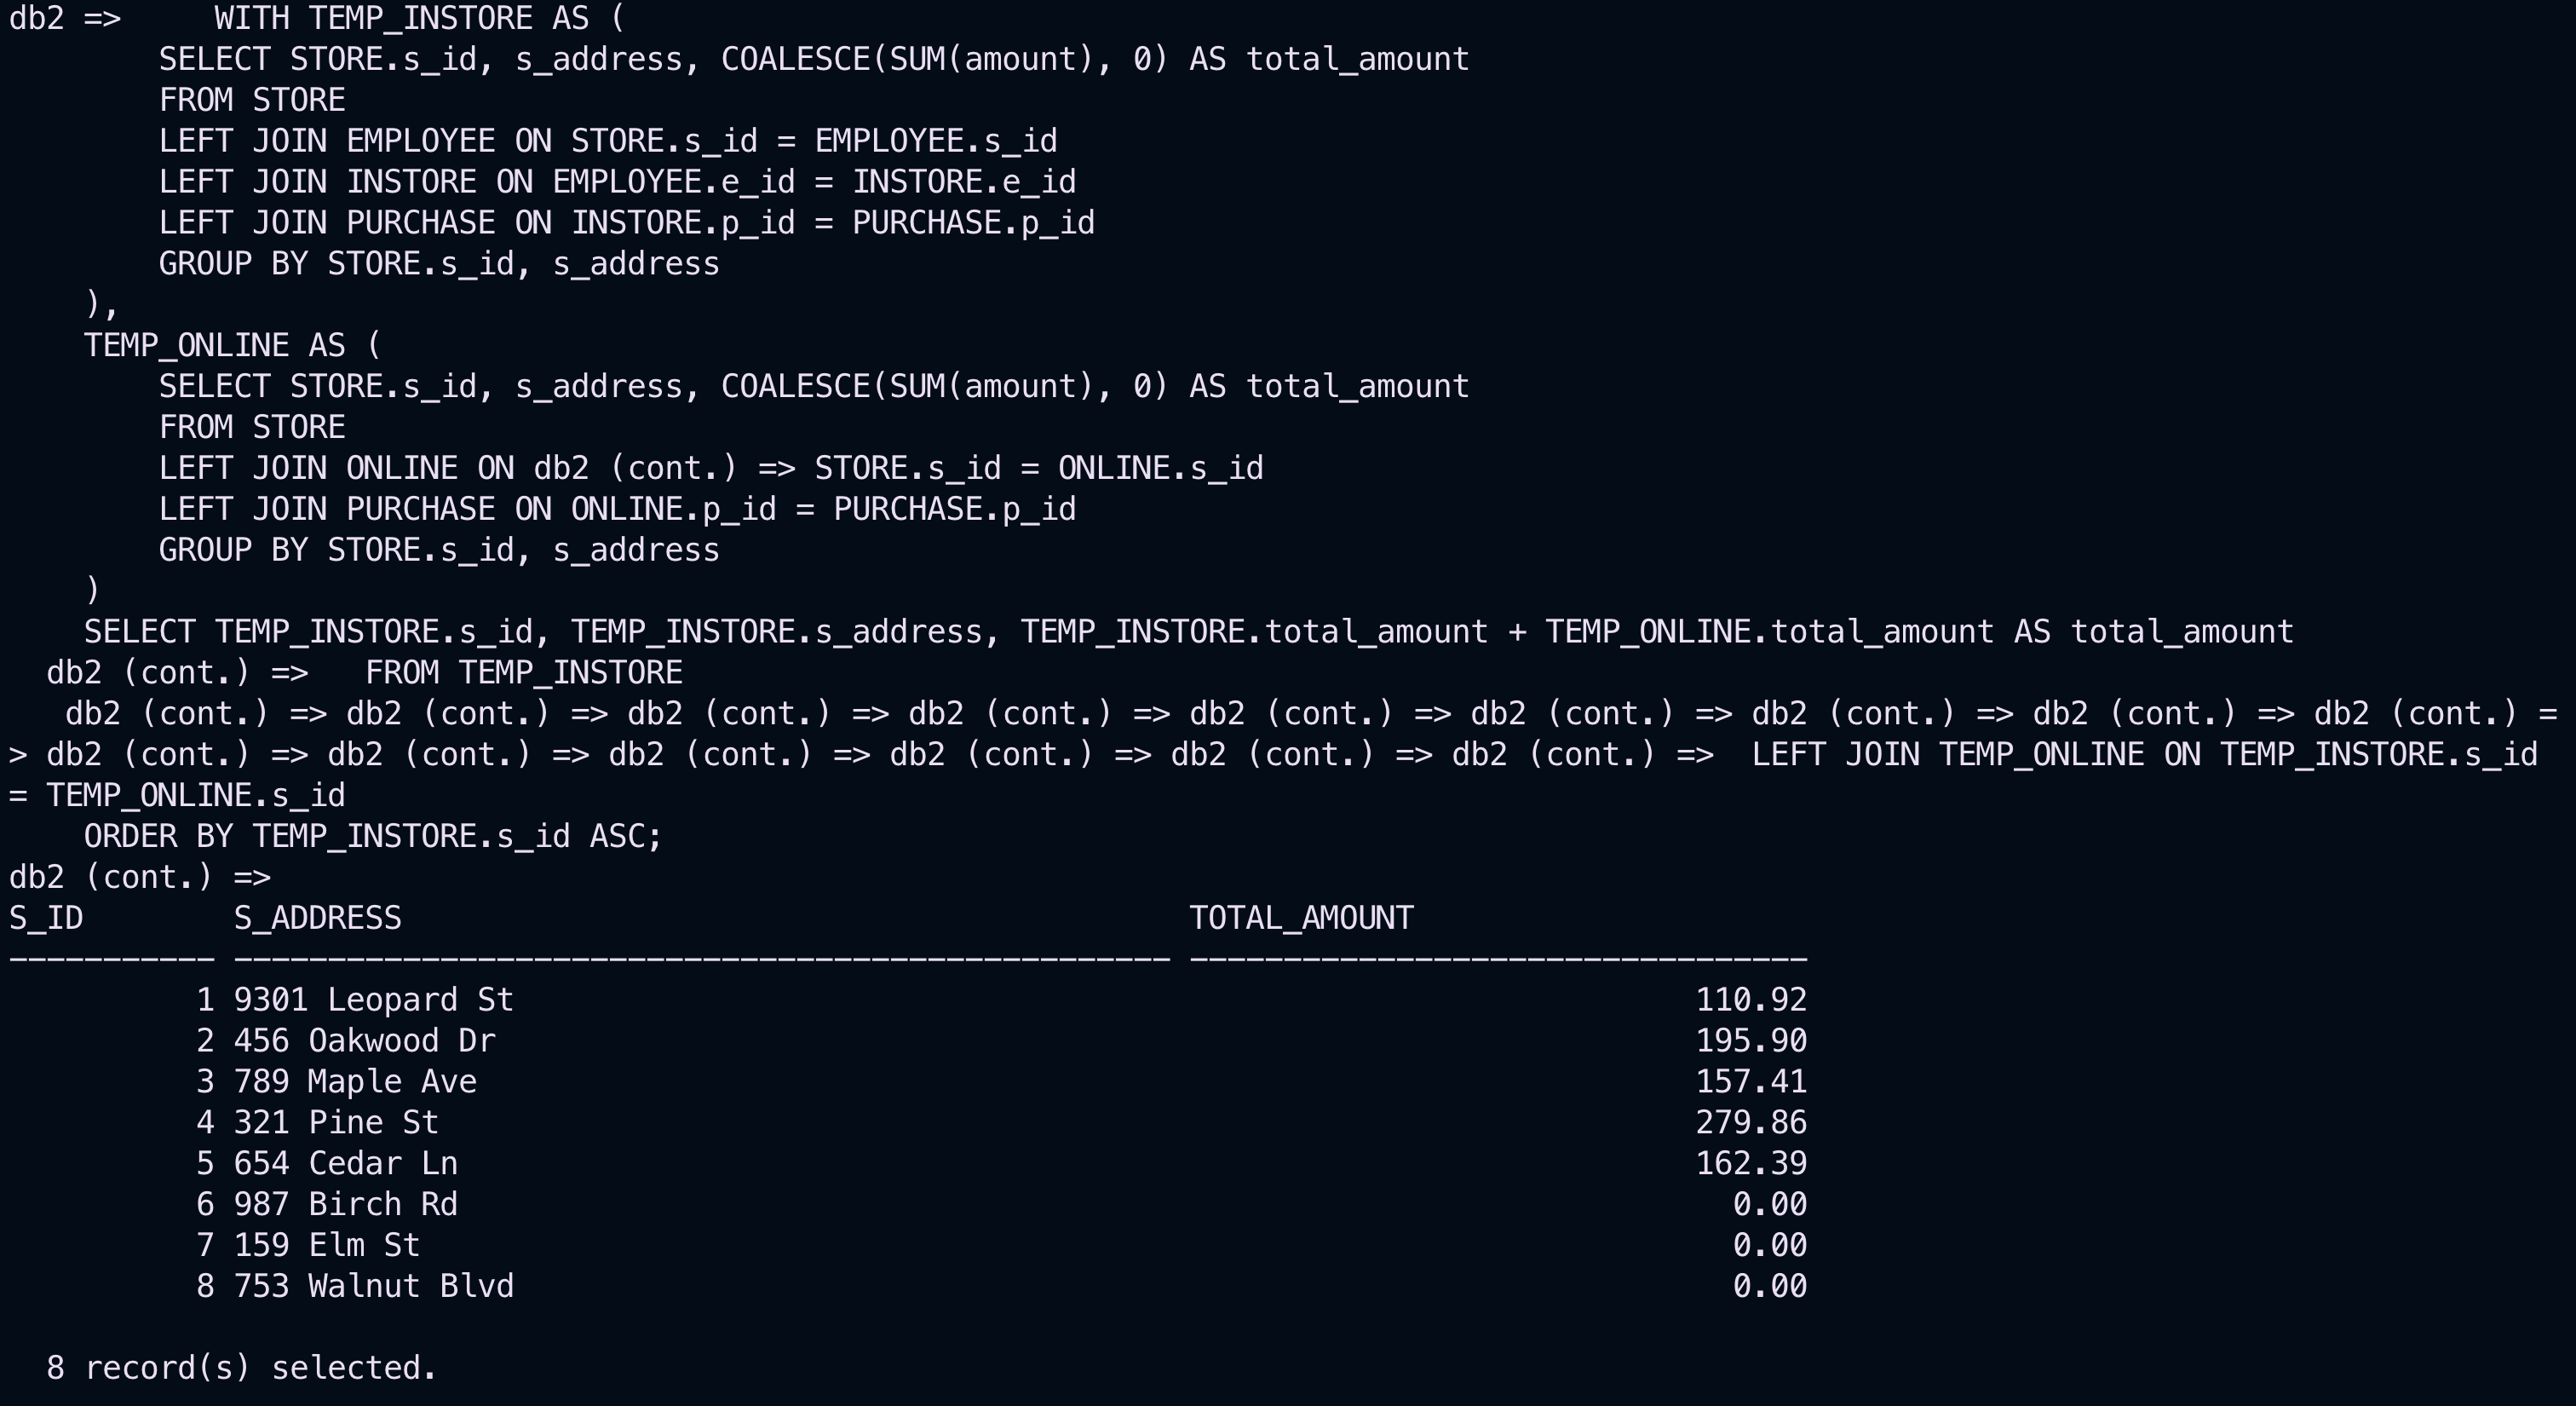
\includegraphics[width=0.8\textwidth]{Query4.png}
    \caption{Query 4 result}
\end{figure}

\subsection*{Query 5}
\begin{enumerate}[label=(\alph*)]
    \item List the Paint products that are in that are in maximum quantity in the store with \\id = 1.
        List the product id, name and quantity.
    \item
        \begin{lstlisting}
        WITH TEMP AS (
            SELECT PRODUCT.p_id, p_name, COALESCE(quantity, 0) AS quantity
            FROM PAINT
            LEFT JOIN PRODUCT ON PRODUCT.p_id = PAINT.p_id
            LEFT JOIN HAS_IN_STOCK ON PRODUCT.p_id = HAS_IN_STOCK.p_id
            WHERE HAS_IN_STOCK.s_id = 1
            ORDER BY quantity DESC
        )
        SELECT p_id, p_name, quantity
        FROM TEMP
        WHERE quantity = (SELECT MAX(quantity) FROM TEMP);
        \end{lstlisting}
    \item
\end{enumerate}
\begin{figure}[H]
    \centering
    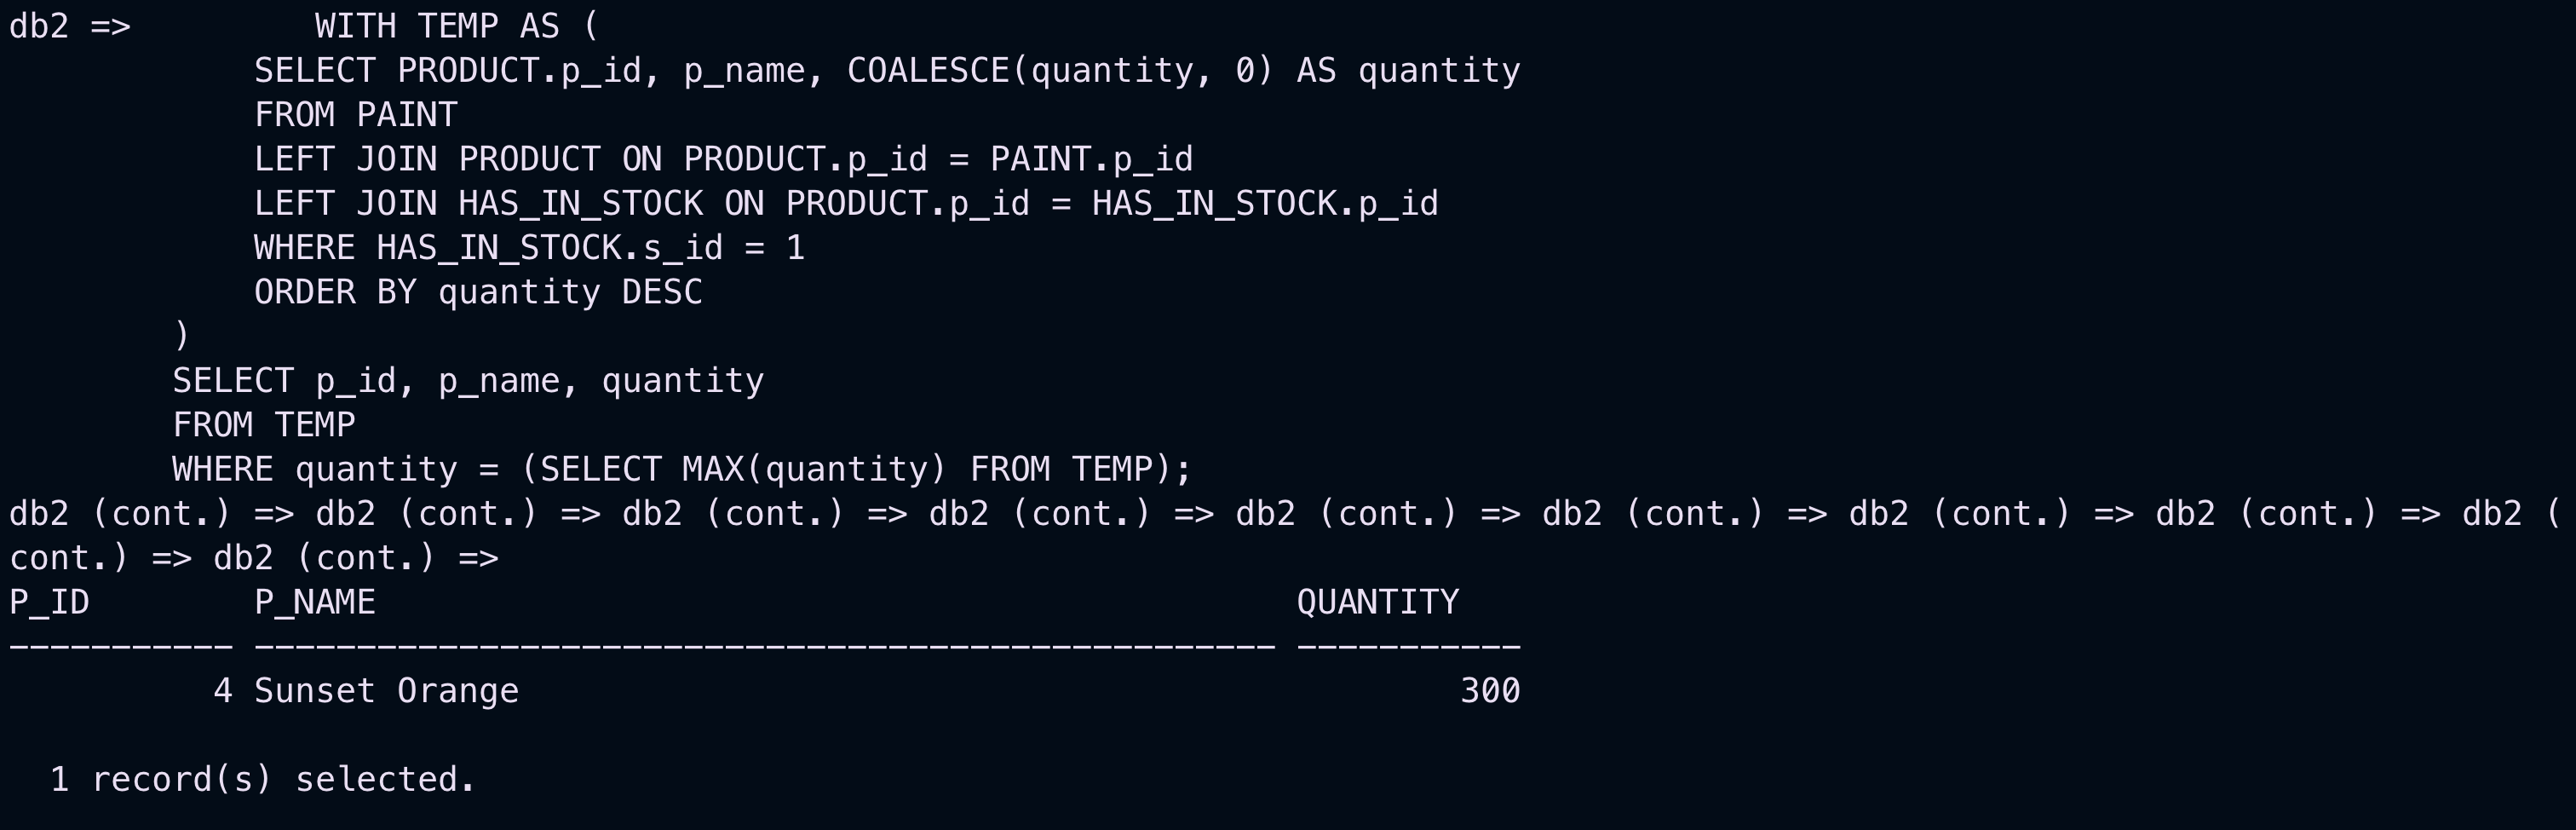
\includegraphics[width=0.8\textwidth]{Query5.png}
    \caption{Query 5 result}
\end{figure}

\section{SQL Modifications}
\subsection*{Mod 1}
\begin{enumerate}[label=(\alph*)]
    \item Temporarily increase the price of products that where manufactured by the manufacturer with name that ends with "Industries" by 10\%.
    \item
        \begin{lstlisting}
        UPDATE PRODUCT
        SET unit_price = unit_price * 1.1
        WHERE m_id IN (
            SELECT m_id
            FROM MANUFACTURER
            WHERE m_name LIKE '%Industries'
        );
        \end{lstlisting}
    \item
\end{enumerate}
\begin{figure}[H]
    \centering
    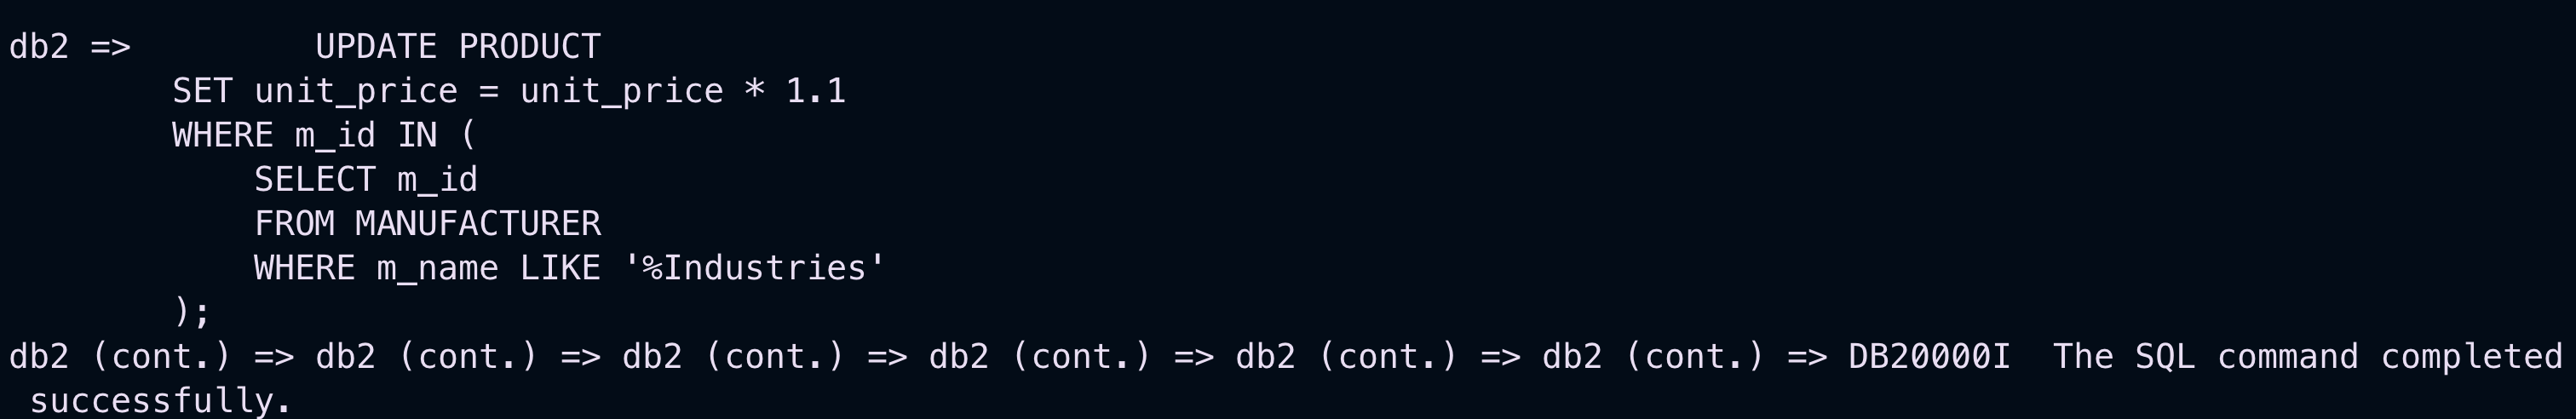
\includegraphics[width=0.8\textwidth]{Mod1.png}
    \caption{Mod 1 result}
\end{figure}

\subsection*{Mod 2}
\begin{enumerate}[label=(\alph*)]
    \item Merge two manufacturers with the id1 = 1 and id2 = 2 into a new manufacturer with name "m\_name1-m\_name2".
    \item
        \begin{lstlisting}
        -- Step 1: Insert a new manufacturer with the combined name
        INSERT INTO MANUFACTURER (m_id, m_name)
        SELECT MAX(m_id) + 1,
               (SELECT m_name FROM MANUFACTURER WHERE m_id = 1) || '-' || (SELECT m_name FROM MANUFACTURER WHERE m_id = 2)
        FROM MANUFACTURER;

        -- Step 2: Update products to assign the new manufacturer (with new m_id)
        UPDATE PRODUCT
        SET m_id = (SELECT MAX(m_id) FROM MANUFACTURER)
        WHERE m_id IN (1, 2);

        -- Step 3: Delete the old manufacturers
        DELETE FROM MANUFACTURER WHERE m_id IN (1, 2);
        \end{lstlisting}

    \item
\end{enumerate}
\begin{figure}[H]
    \centering
    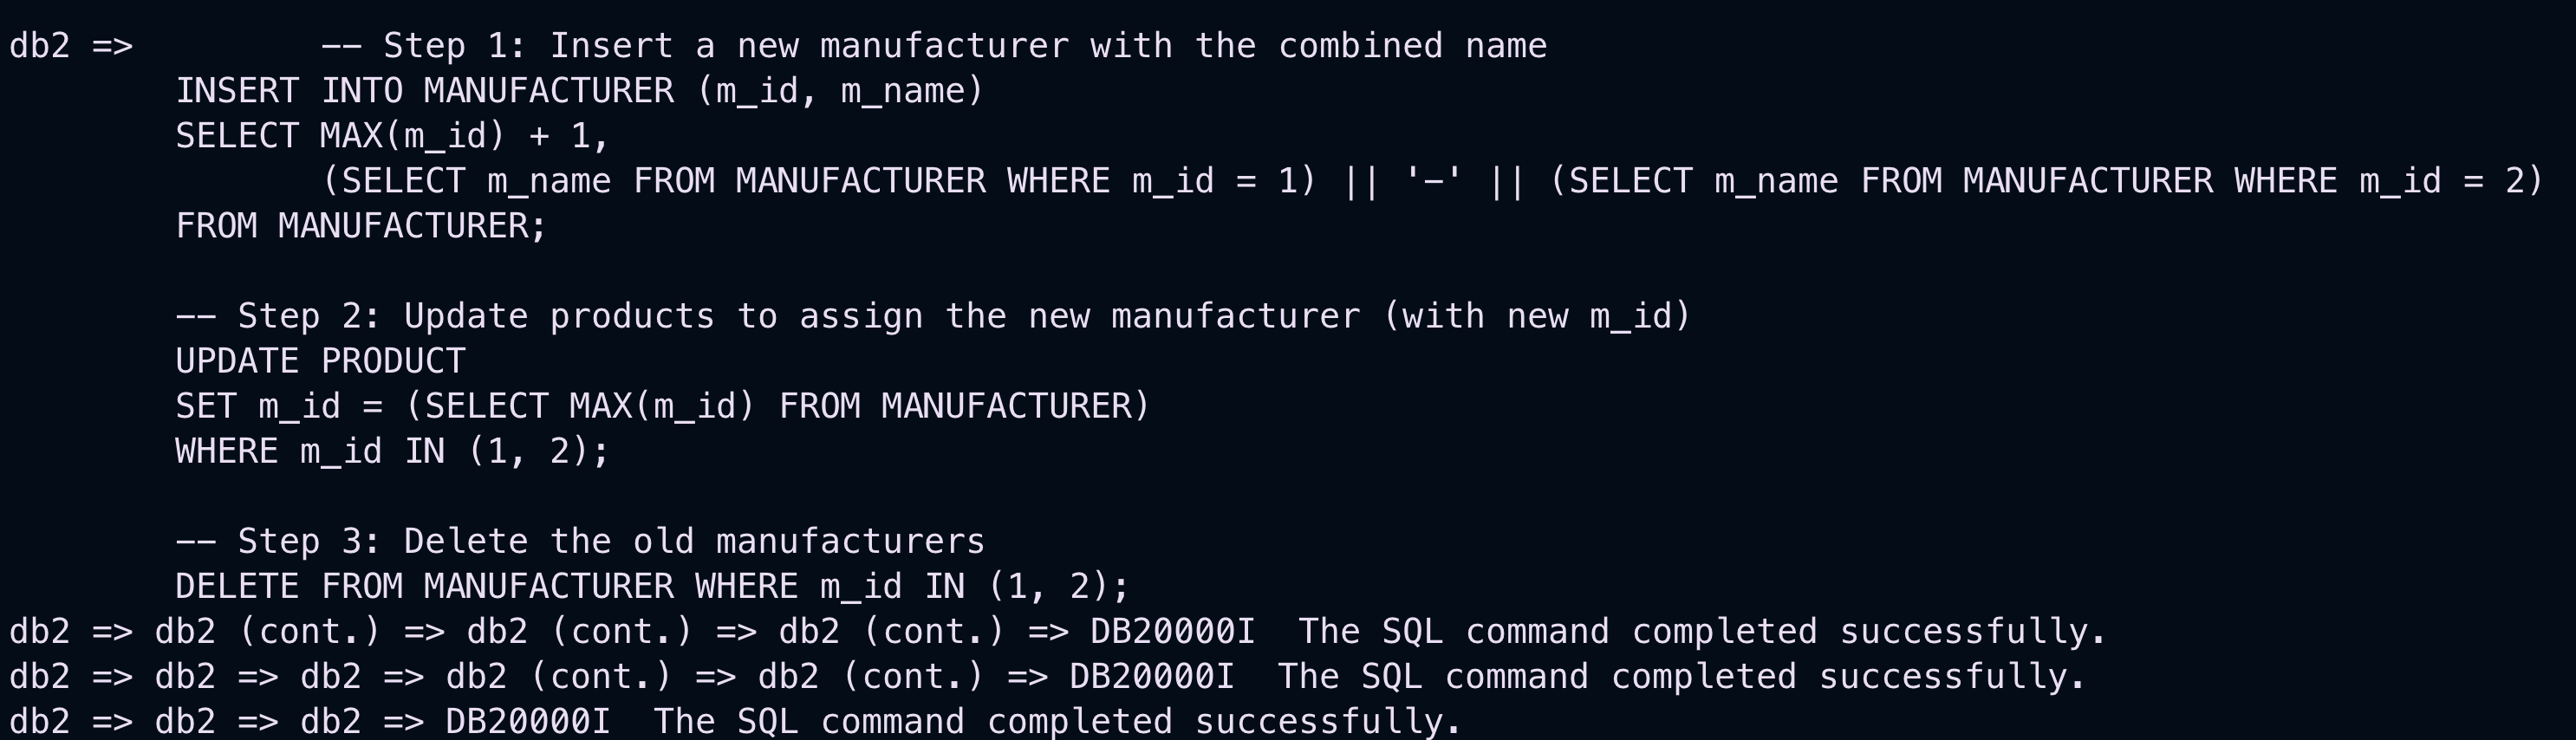
\includegraphics[width=0.8\textwidth]{Mod2.png}
    \caption{Mod 2 result}
\end{figure}


\section{Views}

\subsection*{View 1}

\begin{enumerate}[label=(\alph*)]
    \item The view lists the expensive purchases in descending order of amount, where the amount is greater than or equal to 80.
    \item
        \begin{lstlisting}
            CREATE VIEW EXPENSIVE_PURCHASES AS
            SELECT p_id, amount, p_date, p_time
            FROM PURCHASE
            WHERE amount >= 80;
        \end{lstlisting}
    \item
        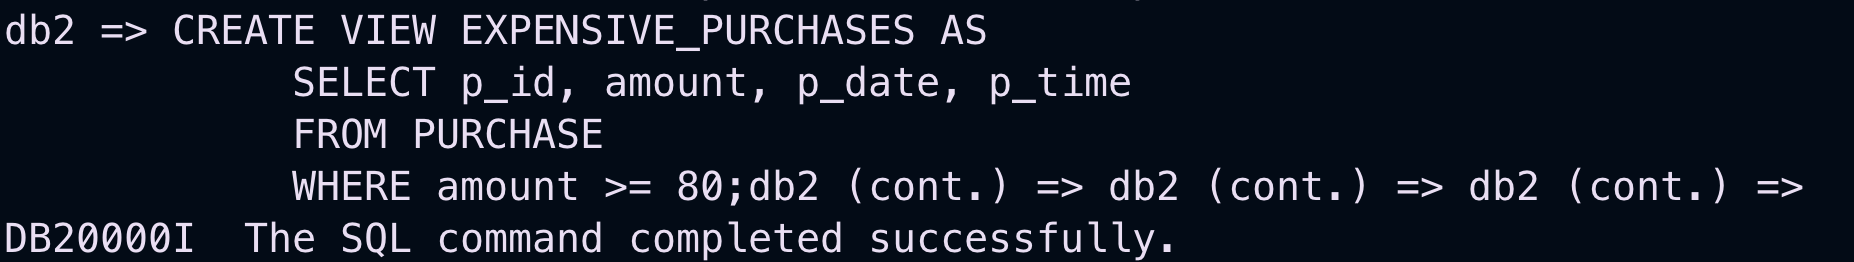
\includegraphics[width=0.8\textwidth]{View1.png}
    \item
        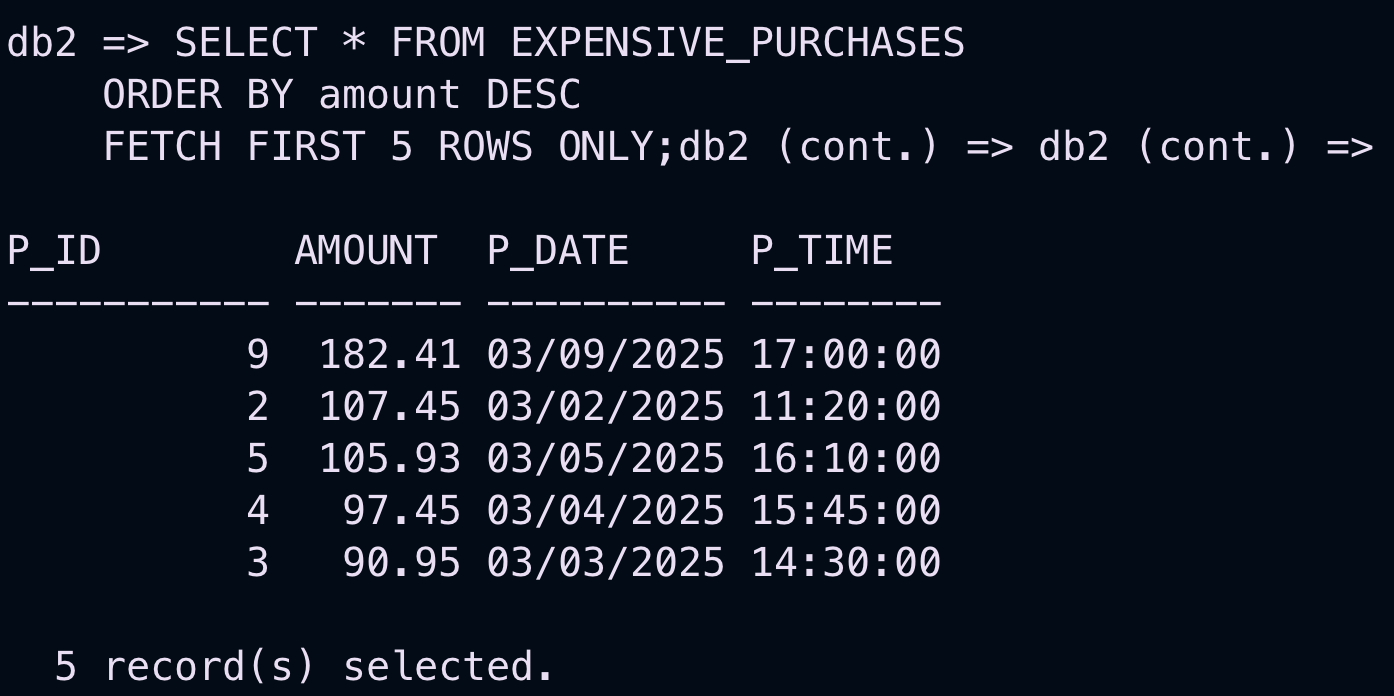
\includegraphics[width=0.8\textwidth]{View1_d.png}
    \item
        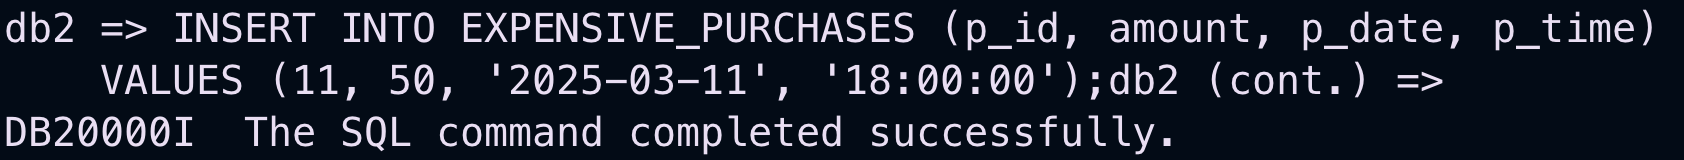
\includegraphics[width=0.8\textwidth]{View1_e.png}
    \item The insertion was completed successfully. However, it is interesting to not that since the amount
    was less than 80, it was not included in the view, and only inserted in the PURCHASE table.
    The explanation for this comes from the following DB manual explanation: For views that are not defined with WITH CHECK OPTION, you can insert rows that do not conform to the definition of the view. Those rows cannot appear in the view but are inserted into the base table of the view.
\end{enumerate}

\subsection*{View 2}
\begin{enumerate}[label=(\alph*)]
    \item This view provides a summary of total amount spent on online purchases by each customer.
    \item
    \begin{lstlisting}
        CREATE VIEW CUSTOMER_ONLINE_SPENDING AS
        SELECT
            Customer.email,
            Customer.c_name,
            COALESCE(SUM(Purchase.amount), 0) AS total_spent
        FROM Customer
        JOIN Online ON Customer.email = Online.email
        JOIN Purchase ON Online.p_id = Purchase.p_id
        GROUP BY Customer.email, Customer.c_name;
    \end{lstlisting}
    \item
        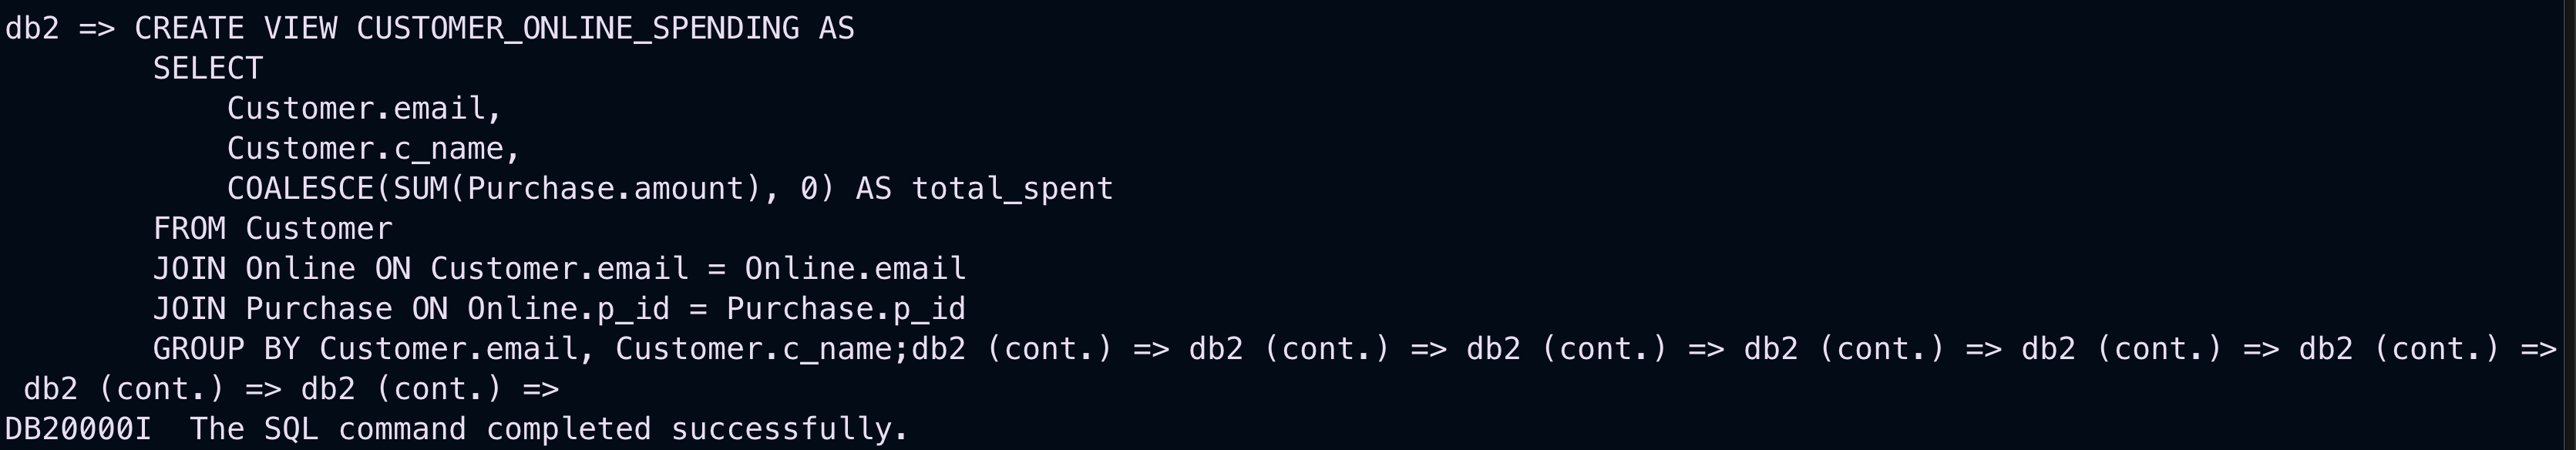
\includegraphics[width=0.8\textwidth]{View2.png}
    \item
        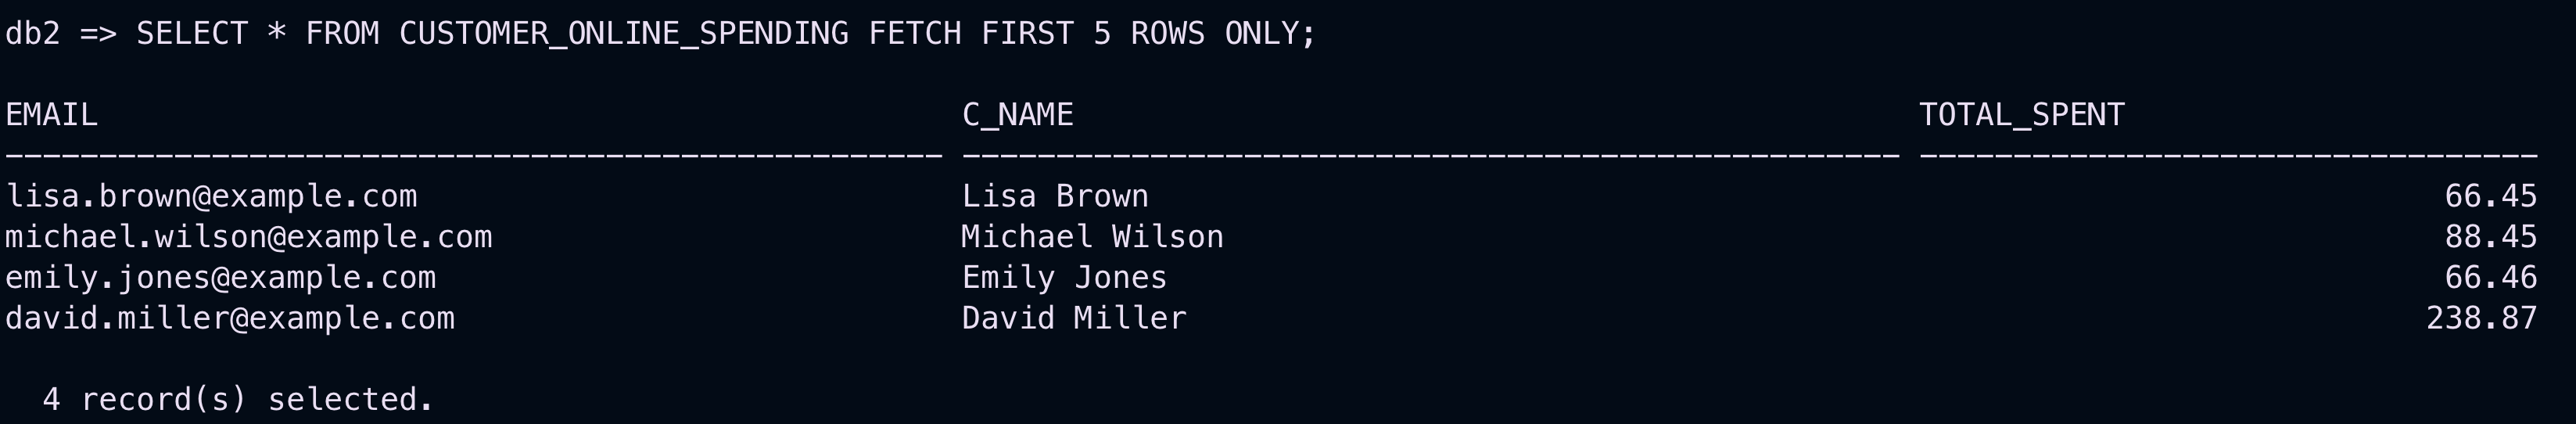
\includegraphics[width=0.8\textwidth]{View2_d.png}
    \item
        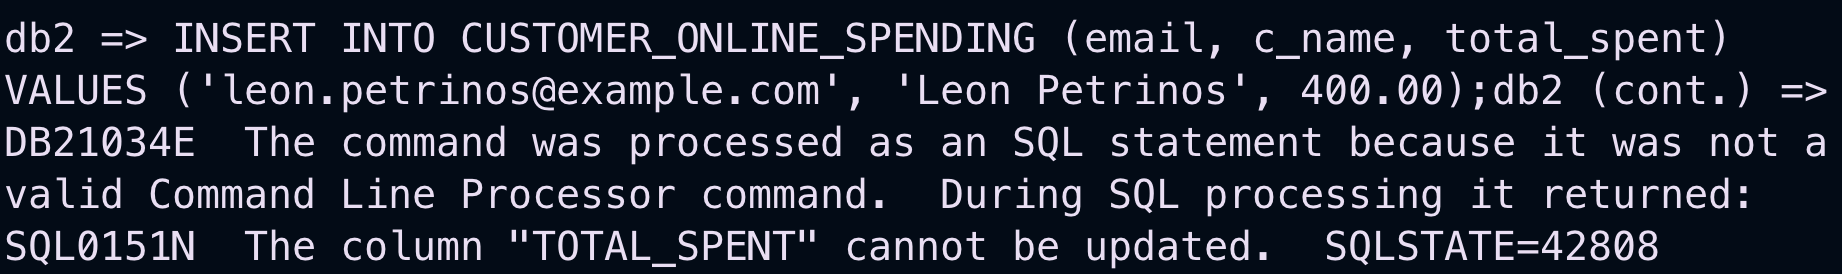
\includegraphics[width=0.8\textwidth]{View2_e.png}
    \item The insert failed with SQLSTATE 42808. The manual states:
    Individual columns in a view cannot be updated if the column is derived from an SQL function, an arithmetic expression, or a constant.
    The TOTAL\_SPENT column is derived from the SUM function, so it cannot be updated.
\end{enumerate}


\section{Check Constraints}
\subsection*{Check 1}
\begin{enumerate}[label=(\alph*)]
    \item The base attribute in the PAINT table should be one of the following: "Gloss", "Matte".
    \item
    \begin{lstlisting}
        ALTER TABLE PAINT
        ADD CONSTRAINT base_check CHECK (base IN ('Gloss', 'Matte'));
    \end{lstlisting}
    \item
        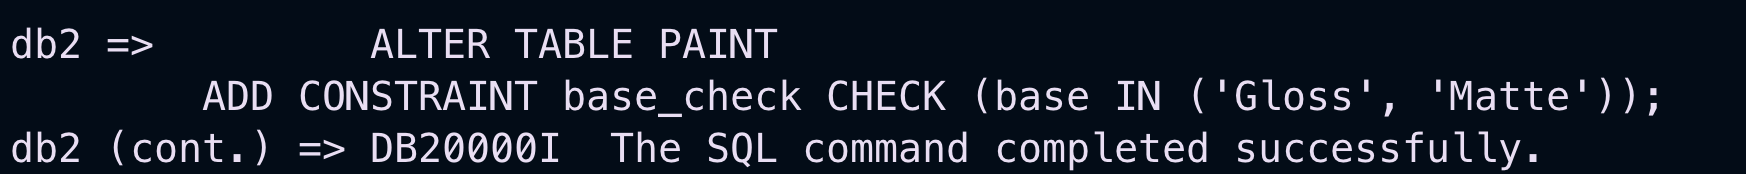
\includegraphics[width=0.8\textwidth]{Check1_c.png}
    \item
        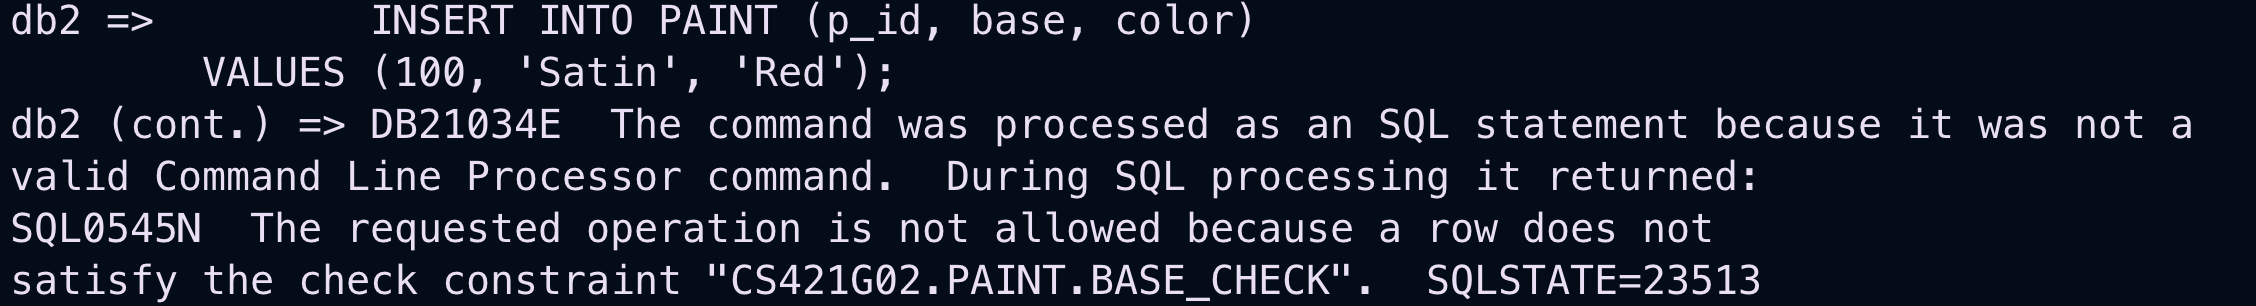
\includegraphics[width=0.8\textwidth]{Check1_d.png}
\end{enumerate}

\subsection*{Check 2}
\begin{enumerate}[label=(\alph*)]
    \item The rating attribute in the ONLINE table should be between 1 and 5 if present otherwise NULL.
    \item
    \begin{lstlisting}
        ALTER TABLE ONLINE
        ADD CONSTRAINT rating_check CHECK (rating BETWEEN 1 AND 5 OR rating IS NULL);
    \end{lstlisting}
    \item
        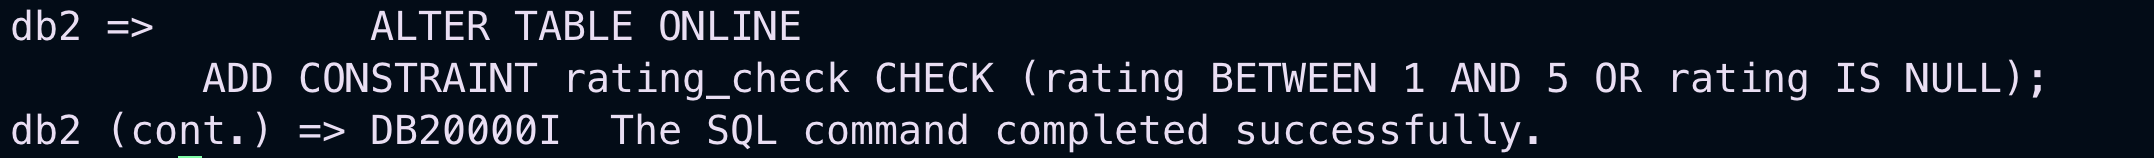
\includegraphics[width=0.8\textwidth]{Check2_c.png}
    \item
        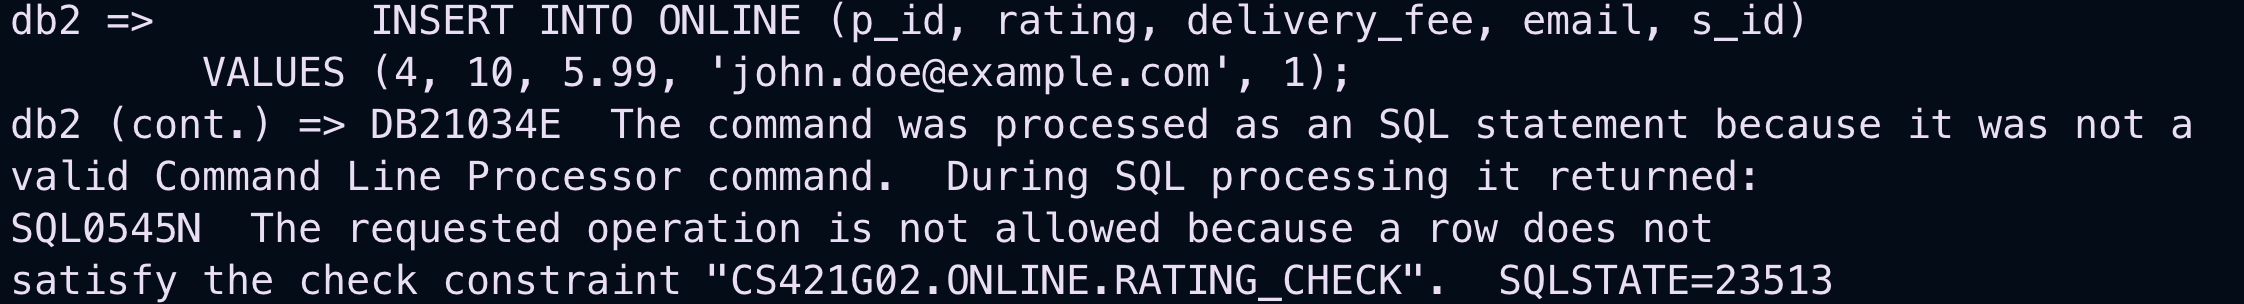
\includegraphics[width=0.8\textwidth]{Check2_d.png}
\end{enumerate}

\section{Creativity}

We decided on option 1 for this question : generating at least one table with meaningful data
for all its attributes.

We generated entries for the Customer table (the Online table has a foreign key to this
table).

To do this, we used an online random name generator (https://1000randomnames.com/)
and an online random address generator (https://quickpseudo.com/generators/person/addressgenerator).
The email addresses were created from the customer name and using a randomly
selected domain name among ”gmail.com”, ”hotmail.com” and ”yahoo.ca”.

We then wrote the insertion operations in software (see Q9.java). The randomly generated
data from the website was copied into .txt files that the program reads from (see random\_names.txt and random\_addresses.txt). The program then randomly picks a domain name
and writes to a file containing all of the insertion operations.

\section{Work Division}
We had two meetings to discuss the project and the work division. We decided to divide the work as follows:
\begin{itemize}
    \item Ahmed Tlili: Relational Schema, questions 4, 5, 6
    \item Leon Petrinos: Relational Schema, question 3, 7, 9
    \item Mathilde Peruzzo: ER Diagram, questions 7, 8, 9
\end{itemize}

\end{document}

